\documentclass[11pt,a4paper]{article}
\pdfoutput=1
%vons grund
\usepackage[utf8]{inputenc}
\usepackage[T1]{fontenc}
\usepackage[german, english, swedish]{babel} %OBS! Se till att vi får rätt språk.
\usepackage{amsmath}
\usepackage{lmodern}
\usepackage{units}
\usepackage{icomma}
\usepackage{color}
\usepackage{graphicx}
\graphicspath{ {bilder/} }
\usepackage{bbm}
\newcommand{\N}{\ensuremath{\mathbbm{N}}}
\newcommand{\Z}{\ensuremath{\mathbbm{Z}}}
\newcommand{\Q}{\ensuremath{\mathbbm{Q}}}
\newcommand{\R}{\ensuremath{\mathbbm{R}}}
\newcommand{\C}{\ensuremath{\mathbbm{C}}}
\newcommand{\rd}{\ensuremath{\mathrm{d}}}
\newcommand{\id}{\ensuremath{\,\rd}}
\usepackage{hyperref}


%%%%%%%%%%%%%%%%%%%%%%%Egna tillägg%%%%%%%%%%%%%%%%%%%%%%%
%%För att få referenser 'på svenska'
%\usepackage[]{babelbib}
%\selectbiblanguage{english}
%\renewcommand\btxauthorcolon{:}
%%För att figurtext i underfigurer
\usepackage{subfigure} 
%%För att kunna inkludera andra PDF-dokument
\usepackage{pdfpages}
%%För att kunna ha roterade bilder
\usepackage{rotating}
%%För att kunna byta uppräkningsvisare t.ex. [label=\alph*)]
\usepackage{enumitem}
%%För att kunna lägga till 'bilagor' utan sidnumrering.
\usepackage{tocstyle}
\usetocstyle{standard}%För att få en vanlig TOC
                %no page numbers for part
\settocstylefeature[-1]{pagenumberbox}{\csname @gobble\endcsname}
\usepackage[nottoc]{tocbibind} %Puts an 'Reference' entry in the ToC.
%%För att kunna använda bra och ket och mycket annat smått och gott
\usepackage{physics} %\bra{}\ket{} eller \expval{H}{\psi}
%%För att kunna rita snygga matriser
\usepackage{mathtools} %\begin{pmatrix*}[r] ... \end
%%För att kunna kommentera ut större stycken
%%Drar in tabell och figurtexter
\usepackage[margin=10 pt, size=small]{caption}
\usepackage{comment} %\begin{comment}
%%För att lägga in 'att göra'-noteringar i texten
\usepackage[]{todonotes} %\todo{...}, \todolist
%\renewcommand{\todo}{\todo {}}

\usepackage{cite}

%%För att inkludera MATLABkod. 
%%OBS: mcode är ett separat paket och man måste ha mcode.sty i samma
%%katalog som dokumentet.
%\usepackage[framed,numbered,autolinebreaks,useliterate]{mcode}
%\usepackage{listings} 
%\lstloadlanguages{matlab} 
%\lstset{language=matlab} 
%\lstset{literate= {å}{{\r{a}}}1 {ä}{{\"a}}1 {ö}{{\"o}}1 {Å}{{\r{A}}}1
%  {Ä}{{\"A}}1 {Ö}{{\"O}}1}%För att få svenska bokstäver från MATLAB.


%%%%%%%%%%%%%%%%%%%%%%%Formatering%%%%%%%%%%%%%%%%%%%%%%%%
%%Partiell derivata
\newcommand{\pd}{\ensuremath{\partial}}
%%Följer ISO-8601 oberoende av språk.
\usepackage[iso, swedish]{isodate}
%%Göra grader Celcius
\newcommand{\degC}{\ifmmode \,^\circ\mathrm{C} \else $\,^\circ\mathrm{C}$ \fi}
%%Figurreferenser
\newcommand{\figref}{\figurename~\ref} 
%%Tabellreferenser
\newcommand{\tabref}{\tablename~\ref} %Stor bokstav i början

%%Det ska vara ett rakt µ i prefixet
\usepackage{upgreek}
\newcommand{\micro}{\upmu}
%%Ohm enhetskommando
\newcommand{\ohm}{\ifmmode \Upomega \else $\Upomega$ \fi}

%%'e' och 'i' ska vara upprätt
\newcommand{\e}{\mathrm{e}}
\newcommand{\ii}{\mathrm{i}}


%%För att själv bestämma marginalerna. 
\usepackage[
%            top    = 3cm,
%            bottom = 3cm,
%            left   = 3cm, right  = 3cm
]{geometry}


\begin{document}

\renewcommand{\thefootnote}{\fnsymbol{footnote}}

%kortkommandon för mailaddresserna
\newcommand{\andsunds}{andsunds@student.chalmers.se}
\newcommand{\rigon}{rigon@student.chalmers.se}



\pagenumbering{roman} %%Romersk sidnumrering i början
\begin{titlepage}
\newgeometry{top=3cm, bottom=2cm}

\newcommand{\HRule}{\rule{\linewidth}{0.5mm}} % Defines a new command for the horizontal lines, change thickness here

\center % Center everything on the page
 
%------------------------------------------------------------------------------------
%	HEADING SECTIONS
%------------------------------------------------------------------------------------

\textsc{\huge Chalmers tekniska högskola}\\[1.5cm] % Name of university/college
\textsc{\Large Rapport, Experimentell fysik 2}\\[0.2cm] % Major heading such as course name
\textsc{\large Termodynamik -- Uppgift 3 }\\[0.5cm] % Minor heading such as course title

%------------------------------------------------------------------------------------
%	TITLE SECTION
%------------------------------------------------------------------------------------

\HRule \\[0.4cm]
{ \LARGE \bfseries 
Studier av kvicksilveratomens atomära emissionsspektra samt absorptionsspektra av laserfärgämnena Rhodamin B och Kumarin 307
}\\[0.4cm] % Title of  document
\HRule \\[1.5cm]
 
%------------------------------------------------------------------------------------
%	AUTHOR SECTION
%------------------------------------------------------------------------------------

\begin{minipage}{0.4\textwidth}
\begin{flushleft} \large
\emph{Författare:}\\
Andréas Sundström\footnotemark{} \\
Rigon Demisai\footnotemark{} 
\end{flushleft}
\end{minipage}
~
\begin{minipage}{0.4\textwidth}
\begin{flushright} \large
\emph{Labassistent:} \\
Martin Wersäll
\end{flushright}
\end{minipage}\\[3cm]

\setcounter{footnote}{0}
\stepcounter{footnote}
  \footnotetext{\href{mailto:\andsunds}{\texttt{\andsunds}}}
\stepcounter{footnote}
  \footnotetext{\href{mailto:\rigon}{\texttt{\rigon}}}



%------------------------------------------------------------------------------------
%	DATE SECTION
%------------------------------------------------------------------------------------
% Följer ISO-standarden för tidsintervall:
% https://en.wikipedia.org/wiki/ISO_8601#Time_intervals
% "Double hyphen" också ok istället för '/'. -- i LaTeX är dock lite på gränsen
{ \large
\begin{tabular}{rc}
    Laboration utförd: & 2015-12-11/15 \\[0.1cm]
    Rapport inlämnad: & \today
\end{tabular}\\[1cm]
}

%------------------------------------------------------------------------------------
%	LOGO SECTION
%------------------------------------------------------------------------------------


\includegraphics[height=5cm]{logo.pdf} % Include a department/university logo
 
%------------------------------------------------------------------------------------

\vfill % Fill the rest of the page with whitespace

\end{titlepage}
\restoregeometry


\setcounter{page}{2}%detta är ANDRA (2) sidan

\renewcommand{\abstractname}{Sammandrag}
\begin{abstract}
Den här rapporten beskriver en spektroskopisk studie av
kvicksilveratomens atomära emissionsspektrum samt en studie av
laserfärgämnena rhodamin~B och kumarin~307 och deras
absorptionsspektra.
Ur emisionspektrumet från Hg har vissa av atomens energinivåer kartlagts,
baserat på kvanmekaniska regler och jämförelse med tidigare data på
Hg.  Kvicksilvrets emissionsspektra
är taget i intervallet 350--1100\,nm, där detekterades totalt 23
emissionstoppar, varefter 13 övergångar kunde identifieras.
Absorptionsspektrumen för rhodamin~B och kumarin~307 visar breda
absorptionsband vilket är kännetecknande för flourescerande ämnen som
består av stora organiska molekyler. 
Mätningarna har utförts med en Spex~270M spektrometer och
datainsamlingen har gjorts i LabView.
\end{abstract}

\renewcommand{\abstractname}{Abstract}
\begin{abstract}
This report describes a spectroscopic study of the atomic emision
spectrum of mercury, and also a study of the laser dyes Rhodamine~D
and Coumarin~307 and their absorption spectrum.
Som of the energylevels of Hg have been idetified from the emission
spectrum, based on quantum mecanichal rules and comparison with erlier
data on Hg. The emission spectrum of mercury was taken in the interval
of 350--1100\,nm, there a total of 23 emission lines were detected,
from which 13 different atomic transitions could be identified. 
The absorption spectrum of Rhodamin~B and Coumarin~307  show wide
absorption bands which are characteristic of big organic molecules.
THe measurements were made with a Spex~270M spectrometer and the data
collection was done through LabVIEW.
\end{abstract}

\clearpage
\renewcommand{\contentsname}{Innehållsförteckning}
\tableofcontents

\clearpage
\pagenumbering{arabic}
\setcounter{page}{1}

\renewcommand{\thefootnote}{\arabic{footnote}}
\setcounter{footnote}{0}





\section{Inledning}
Spektroskopi har varit, och är fortfarnde, ett kraftfullt verktyg för
exempelvis kemister och astronomer för att avgöra vad för grundämnen
och molekyler som undersöks. Tack vare att alla grundämnen har sina
egna emissions- och absorptionsspektra har man utan direkt
tillgång till en substans kunnat avgöra dess innehåll genom dess
spektrum. 

Dessa spektra består vanligen av distinkta linjer. Och det beror på
att elektronerna bara kan ha vissa diskreta energinivåer i atomen. Så
är i alla fall fallet med \emph{atom}spektran. Men om större molekyler
undersöks så finns ofta många tätt liggande nivåer så att
spektrallinjerna blir ''utsmetade''. Detta är fallet med
t.ex. laserfärgämen -- ämnen som absorberat en kortare ljusvåglängd
och sedan via olika mellansteg emitterar ljus med en längre våglängd.

Bestämming av vilka ämnen som finns i ett prov må vara bland de
vanligaste tillämpningarna av spektroskopi. Men den här rapportens
syfte är att dels bestämma ett energinivådiagram från ett
atomspektrum, dels observera och förklara absorptionsspektrat från två
laserfärgämnen.  Denna rapport kommer specifikt studera
emissionspektrat för kvicksilver\footnotemark{} och
absorptionsspektrumen från två laserfärgämne och utifrån det
konstruera motsvarande energinivådiagram. 
\footnotetext{Anmärkning: Det var egentligen sagt att vi skulle
  undersöka kadmium, men kadmiumlampan (eller aggregatet till den
  typen av spektrallampor) gick sönder när mätningarna skulle
  starta. På grund av att laborationen utfördes över en helg gick det
  inte att ersätta spektrallampan, så en annan lampa (med ett annat
  aggregat) fick användas istället. Så kvicksilver valdes som en
  ersättare, utan egentlig eftertanke. }


\subsection{Tillämpning på kvicksilver (icke-joniserat)}
I fortsättningen av denna rapport förutsätts att läsaren är bekant med
den kvantfysik och de vanligaste benämningar som förekommer i studiet
av atomer. Om så inte är fallet finns en kortare genomgång om detta i
Bilaga~\ref{sec:teori}.

Kvicksilvers grundkonfiguration är $6\mathrm{s}^2$, vilket betyder att det
finns två valenselektroner med $n=6$ och $l=0$ för de båda. Utav dessa
två antas en av dem kunna exciteras till en högre energinivå (högre
$l$ eller $n$), medan den andra stannar i 6s-tillståndet. 

Detta är en rimlig approximation eftersom det är de excitationerna
med lägst energi. Om båda elektronerna hade exciterats till högre
energier blir det inte bara en fördubbling av energi för att
det blir två elektroner på de högre nivåerna. Det blir dessutom extra
energi på grund av att den andra elektronen blir hårdare bunden till
kärnan, när en elektron redan exciterats. 

I \tabref{tab:Hg_termer} visas några av kvicksilvers
elektronkonfigurationer tillsammans med motsvarande termer. Man kan då
till att börja med försöka sortera dem med hjälp av bland annat Hunds
regler. 
Med hjälp av urvalsreglerna ovan kan man utifrån dessa termer sedan 
ta fram ett antal möjliga övergångar som förhoppningsvis kan paras ihop
med observerade spektrallinjer. 

\begin{table}
\centering
\caption{Tabell med de spektroskopiska termerna för några av de lägsta
exciterade tillstånden för Hg-atomen. Anledningen till att det bara
finns en $L$-term per konfiguration  är att den elektron
som inte exciterats är i ett s-tillstånd, vilket motsvarar $l=0$.}
\label{tab:Hg_termer}
\begin{tabular}{|l|l|l|}\hline
Konfiguration & Singletter ($S=0$) & Tripletter ($S=1$)
\\ \hline\hline
6s6s (grundtillstånd) & $6^1\mathrm{S}_0$ & --- \\ 
\hline
6s6p & $6^1\mathrm{P}_1$ & $6^3\mathrm{P}_J$, $J=2, 1, 0$ \\
6s6d & $6^1\mathrm{D}_2$ & $6^3\mathrm{D}_J$, $J=3, 2, 1$ \\
6s6f & $6^1\mathrm{F}_3$ & $6^3\mathrm{F}_J$, $J=4, 3, 2$ \\
(6s6g) & $6^1\mathrm{G}_4$ & $6^3\mathrm{G}_J$, $J=5, 4, 3$ \\
\hline
6s7s & $7^1\mathrm{S}_0$ & $7^3\mathrm{S}_J$, $J=1$ \\
6s7p & $7^1\mathrm{P}_1$ & $7^3\mathrm{P}_J$, $J=2, 1, 0$ \\
6s7d & $7^1\mathrm{D}_2$ & $7^3\mathrm{D}_J$, $J=3, 2, 1$ \\ 
\hline

\end{tabular}
\end{table}

\subsubsection{Termerna ordnade i energiordning}
Genom att, från avsnitt~\ref{sec:regler}, först utnyttja
Madelungreglen och sedan Hunds regler kan man göra en uppskattning om
i vilken ordning varje term kommer. Hela den uppskattade listan visas
i \tabref{tab:sorterade_termer}, i Bilaga~\ref{sec:kompl}.

En sak som däremot kan sägas är att ju högre upp i energi man kommer
desto närmare varandra kommer nivåerna. Alltså att det med största
sannolikhet är större skillnad mellan grundtillståndet och första
exciterade nivån än mellan resten av de exciterade nivåerna. 

Vidare kan man från avsnitt~\ref{sec:LS} dra slutsatsen att
spinn-banuppsplittringen är störst för de tillstånd som i medel
befinner sig närmast kärnan. Vilket man kan anta är de med lägst
(ouppsplittrad) energi och lägst $l$-kvanttal.\footnotemark{} Alltså
att exempelvis $6^3\mathrm{P}_J$-tillstånden har betydligt större
uppsplittring än $6^3\mathrm{D}_J$-tillstånden som både har högre
energi och högre $l$-kvanttal.  
%Eftersom $\Delta E_\text{SB} \propto\ev{r^{-3}}$ kan man nog till och
%med anta att uppsplittringen är obetdlig för $6^3\mathrm{D}_J$
%jämfört med $6^3\mathrm{P}_J$.
\footnotetext{Det är mer komplicerat än bara ''lägst'' av det ena eller
  det andra. T.ex. styr $l$-värdet på en viss orbital starkt hur
  elektronens radiella sannolikhetsfördelning ser ut.} 


\subsubsection{Att bestämma energinivåer från ett emissionsspektrum}
\label{sec:teori_nivaer}
Från det uppmätta spektrat kunde ett antal toppar identifieras. Givet
dessa toppar kan man sedan direkt identifiera ett antal olika
energinivåskillnader. 

Därefter kan man utgå från en mer eller mindre ordnad lista,
exempelvis \tabref{tab:sorterade_termer} i Bilaga~\ref{sec:kompl},
över LS-termer och antaganden om spinn-banuppsplittringens storlek
samt urvalsreglerna för att försöka hitta toppar eller grupper av
toppar som hör till vissa grupper av energinivåer. 
Tyvärr är enbart dessa regler och metoder inte tillräckliga för att
entydigt bestämma energinivåerna. Men man kan åtminstone komma fram
till och troliggöra några hypoteser. Därefter får man konsultera
referensverk med kända värden på energinivåerna, och utifrån detta
anpassa de egna observationerna.

\paragraph{Grundtillståndet}
En sådan sak, som går att teoretiskt försöka förutsäga, är huruvida
ens mätningar innehåller övergångar ner till grundnivån. De största
stegen i energi är, med strörsta sannolikhet, de som går ner till
grundtillståndet. Vidare är $\mathrm{P}_1$-tillstånden de enda som har
tillåtna övergångar till grundnivån ($6^1\mathrm{S}_0$).

För varje $n$ finns det två $\mathrm{P}_1$-tillstånd -- 
$(2S +1) = 1, 3$. De lägsta av dess är de för $n=6$. Nästa sådant
tillstånd kommer ha en märkbart högre energi. Detta leder nu till
slutsatsen att om man har med spektraltoppar från övergångar ner till
grundnivån, så kommer sådana toppar att vara de med \emph{kortast
  våglängd} och komma i \emph{par om två} (möjligtvis ganska brett
emellan).


\section{Metod}
Spektroskopi är en ganska rätt fram metod. Man har ett prov som man
kan erhålla ljus ifrån. Ljuset leds sedan in i en monokromator som
plockar ut en specifik våglängd åt gången. Monokromatorn kan sedan
variera vilken våglängd som plockas ut. Detta möjliggör mätning av
ljusintensiteten för de våglängder man är intresserade utav. På så
sätt fås spektrumet fram.

\subsection{Spektrometern}

Spektrometern som användes, en Spex~270M \cite{Spex270M}, hade all
nödvändig optisk mät- och styrutrusting inbyggt. Allt som behövde
göras var att koppla upp den, via GPIB, till ett egenkonstruerat
styrprogram i LabVIEW 
för att styra våglängd från monokromatorn och spaltbredd för
ljusinsläppet. Sedan kopplades signalen från fotomultiplikatorn i
spektrometern till en nanoamperemeter som kunde detektera den svaga
strömmen. Nanoamperemetern konverterade strömmen till en spänning som
kunde mätas av en digital multimeter kopplad till styrprogrammet via
GPIB. 

Spektrometern hade inbyggd våglängdsavläsning, men den behövde
kalibreras inför varje mätning. För att göra detta användes en
natriumlampa och natriumets två starka toppar vid 589,0\,nm och
589,6\,nm för att kalibrera den avlästa våglängden. Egentligen
användes bara den ena toppen för att kalibrera, men man kunde utnyttja
den kända våglängdsskillnaden mellan Na-topparna för att identifiera
rätt toppar. 


\subsection{Kvicksilverspektrum}
För att få en så bra noggrannhet i energi som möjligt måste man
maximera sin noggrannhet i våglängd. Spektrometern hade en minsta
våglängds\emph{steglängd}\footnotemark{} på 0,03\,nm. Dock tar varje
intensitetsmätning cirka 5\,s, vilket gör att en
genomlöpng av hela mätintervallet på högta upplösningen skulle ta i
storleksordningen fem timmar. 
\footnotetext{Ej att förväxla med våglängds\emph{upplösningen} i en
  mätning.} 

För att minska körtiden för en mätning skrevs ett program som gick
fram med steg om 1\,nm. Men för att få bra noggrannhet i topparnas
position användes ett tröskelvärde. Så varje gång intensiteten steg
över detta tröskelvärde backade spektrometern ett steg och började gå
med minsta möjliga våglängdssteg. 

Spaltbredden för det insläppta ljuset hölls dock hela tiden
konstant på (0,10\,mm). Detta eftersom den, förutom
våglängdsnoggrannheten, även styr intensiteten på det detekterade
ljuset. Så för att inte få problem med olika intensitet i de olika
mätlägena hölls spaltbredden konstant. 

\subsubsection{Energinivåbestämming}
För att bestämma energinivåerna kan man, till att börja med, utgå från
resonemangen i avsnitt~\ref{sec:teori_nivaer}. Det kan, med viss
osäkerhet, ge några energivåer, men det är svårt att på det viset
lyckas koppla alla topparna man finner med övergångar. 

Det som presenterades i avsnitt~\ref{sec:teori_nivaer} är grunden till
metodiken för att bestämma energinivåer utan någon tidigare vetskap om
dem. Men i vårt fall finns nuförtiden redan känd data på
energinivåernna till kvicksilver. Det går alltså att utgå från redan
kända energinivåer och därifrån se om man kan matcha de uppmätta
topparna med dessa nivåer. 


\subsection{Absorption i lösningar}

För att studera absorptionsspektret från ett prov är grundtanken
ganska enkel: man lyser en lampa med känt spektrum på provet och ser
\href{https://xkcd.com/1517/}{hur det transmitterade ljuset skiljer
  sig från ursprungsspektrumet}. I verkligheten behöver man vara lite
mer vaksam. 

Man får börja med att ta upp ett bakgrundsspektrum från den lampa man
använder för att lysa igenom provet. Därefter kan man göra sin mätning
med provet på plats. Då bakgrundsspektrumet inte var en konstant
intensitet i alla delar av våglängdsintervallet jämfördes de olika
spektrumen genom att undersöka \emph{kvoten} mellan intensiteterna med
och utan prov. Dessutom gjordes fem svep genom hela spektrumet för
varje prov, för att kunna ta ett medelvärde och minska bruset i datan. 


\section{Resultat}
Resultaten från de spektroskopiska mätningarna visas i form av
spektrum från kvicksilverlampan och absorptionsmätningarna i
figurerna~\ref{fig:Hg_spektrum} respektive \ref{fig:absorption}.

I \figref{fig:Hg_spektrum} finns dels det uppmätta spektrumet från
spektrallampan, dels vilka toppar som borde finnas enligt en lista
från NIST~\cite{NIST_spectrum}, dels vilka toppar som detekterats. Man
kan notera att det som kan se ut som \emph{en} topp i bilden faktiskt
är flera vilket syns bland de utmarkerade topparna.

Från spektrallinjerna i \figref{fig:Hg_spektrum} kan man sedan
rekonstruera energinivåerna med hjälp från redan känd data om
kvicksilvers energinivåer~\cite{NIST_levels}. Resultatet från denna
rekonstruktion visas i \tabref{tab:Hg_nivaer}.
För en detaljerad lista över vilka våglängder och energier, tillsammans
med motsvarande övergång, som detekterades för topparna i
kvicksilverspektrumet hänvisas läsaren till \tabref{tab:Hg_toppar} i
Bilaga~\ref{sec:kompl}. 


%% I \figref{fig:svartkropp} visas det uppmätta spektrat från en
%% (halogen) glödlampa. \figref{fig:svartkropp} visar även
%% intensitetsfördelningen från Plancks stråningslag. För att kompensera
%% för skillnaden i känslighet hos spektrometern användes en
%% korrektionsfakor i \figref{fig:Hg_spektrum}. Mer om hur
%% korrektionsfakorn beräknades finns i \appendixname~\ref{sec:korr}.

I \figref{fig:absorption} visas absortionsspektrumen från rohdamin~B
och kumarin~307 i form av kvoten mellan den absorberade intensiteten
och bakgrundsintensiteten. Man kan se två absortionsdalar för båda
ämnena. En annan sak att notera 
är att åtminstone för kumarinet kan man märka en liten ökning i
intensitet vid våglängderna närmas efter en absorptionsdal. 

Vidare syns att rhodamin~B exciteras i ett spektralband som
sträcker sig från cirka 470 till 580\,nm; med maximal
excitation/absoption vid ungefär 540\,nm. Åt höger i grafen finns ett
andra excitationsmaximum vid cirka 1080\,nm i området av ett något
bredare absorptionsband. Notera hur den andra dalen verkar ligga vid
ungefär dubbla våglängden jämfört med den första. 

Kumarin~307 har från vänster i grafen ett absorptionsband
mellan 330 och 470\,nm med ett excitationsmaximum vid ungefär 430\,nm. Det
andra excitationsmaximat finns vid cirka 880\,nm, som också ligger
nära dubbla våglängden från den första absorptionsdalen. 


\begin{sidewaysfigure}
\centering
\centerline{ %centrerar även större bilder
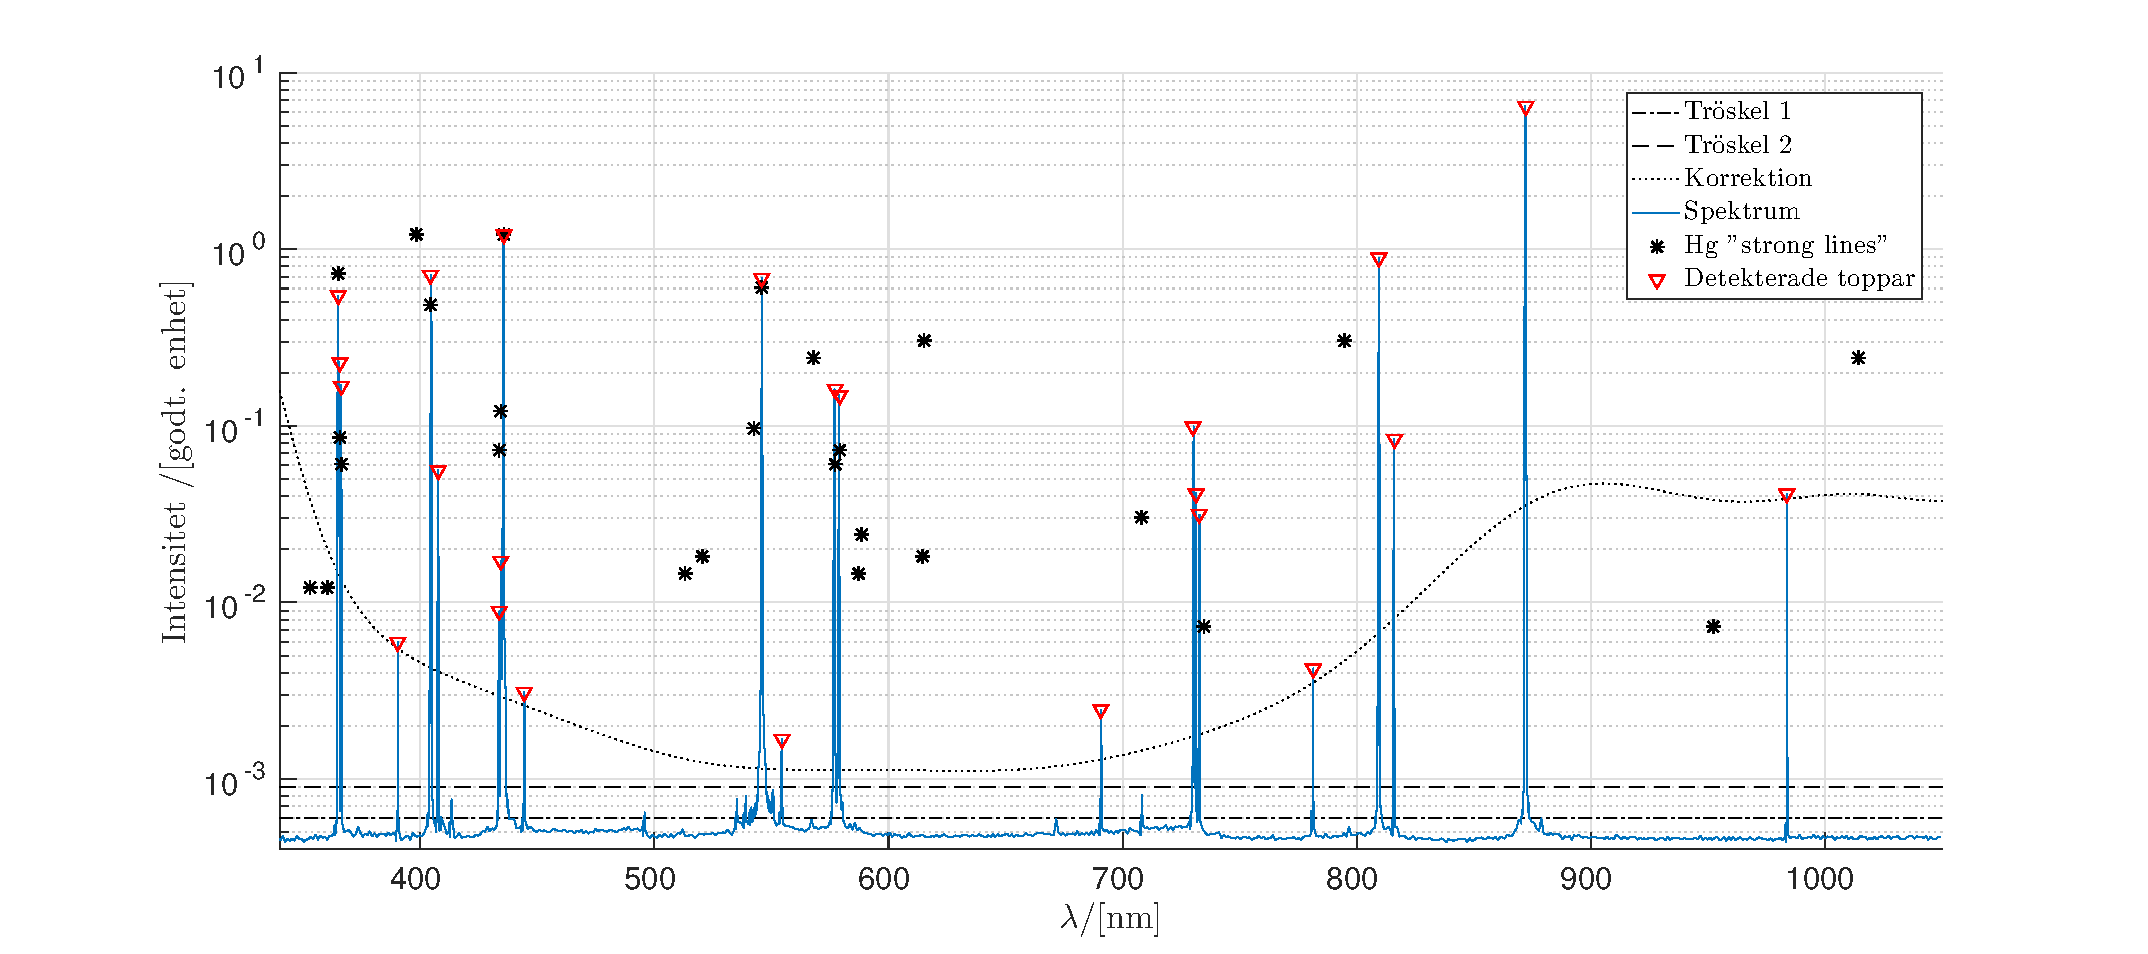
\includegraphics[width=1.2\textwidth]{Hg_spektrum.pdf}
}
\caption{Spektrum uppmätt från kvicksilverlampa tillsammans med
  utmarkerade spektraltoppar enligt NIST\cite{NIST_spectrum}. 
  De tabellerade topperna kallas ''strong lines'' av NIST.
  Av de två trösklarna som är utritade, styr den första när en en topp
  ska anses stor nog för att det ska vara intressant att minska
  steglängden i våglängd, och den andra tröskeln styr när korrektionen
  ska användas. Korrektionen används bara för de toppar som når över
  den andra tröskeln för att inte den bredare basen på en topp ska
  orsaka att hela toppen ser onaturligt bred ut. Notera att intensiteten
  är ritad med log-skala, vilket gör att korrektionsfaktorn effektivt
  adderas till toppens höjd varför korrektionen är utritad relativt
  tröskelvärdet och alltså inte spegler värdet som ges på
  intensitetsaxeln. 
}
\label{fig:Hg_spektrum}
\end{sidewaysfigure}

\begin{table}
\centering
\caption{Lista över energinivåer som detekterats ur spektrumet i
  \figref{fig:Hg_spektrum}. Notera här hur de flesta av de uppmätta
  energinivåerna ligger inom den uppsakttade osäkerhetsgränsen, på
  0,05\,\%, från de tabellerade värdet från NIST
  \cite{NIST_levels}. Energierna är angivna relativt grundtillståndet
  $6^1\mathrm{S}_0$. Eftersom inga övergångar till grundtillståndet
  förekom i spektrat har $6^3\mathrm{P}_0$ i de egna mätningarna satts
  till NIST:s värde. } 
\label{tab:Hg_nivaer}
\begin{tabular}{|c||c|c|c|c|c|}\cline{2-6}
\multicolumn{1}{c|}{} &
\multicolumn{2}{|c|}{Dessa mätningar} & 
\multicolumn{2}{|c|}{Enligt NIST\cite{NIST_levels}} 
& Avvikelse från NIST
\\ \cline{2-6}
\multicolumn{1}{c|}{} &
\unit{eV} 
& $\unit[10^3]{cm^{-1}}$ &\unit{eV} 
& $\unit[10^3]{cm^{-1}}$
& \%
\\ \hline
$6^1\mathrm{S}_0$ &0 & 0 & 0 & 0 & ---
\\ \hline
$6^3\mathrm{P}_0$ &4,667 & 37,64 & 4,667 & 37,64 & --- \\ \hline 
$6^3\mathrm{P}_1$ &4,885 & 39,40 & 4,886 & 39,41 & 0,03 \\ \hline 
$6^3\mathrm{P}_2$ &5,460 & 44,04 & 5,461 & 44,04 & 0,01 \\ \hline 
$6^1\mathrm{P}_1$ &6,705 & 54,08 & 6,704 & 54,07 & 0,01 \\ \hline 
$7^3\mathrm{S}_1$ &7,731 & 62,36 & 7,730 & 62,35 & 0,01 \\ \hline 
$7^1\mathrm{S}_0$ &7,709 & 62,18 & 7,926 & 63,93 & 2,74 \\ \hline 
($6^1\mathrm{D}_2$) &8,846 & 71,35 & 8,844 & 71,33 & 0,02 \\ \hline 
$6^3\mathrm{D}_1$ &8,846 & 71,35 & 8,845 & 71,34 & 0,02 \\ \hline 
$6^3\mathrm{D}_2$ &8,854 & 71,41 & 8,852 & 71,40 & 0,02 \\ \hline 
$6^3\mathrm{D}_3$ &8,858 & 71,44 & 8,856 & 71,43 & 0,02 \\ \hline 
$8^3\mathrm{P}_2$ &9,526 & 76,83 & 9,525 & 76,82 & 0,01 \\ \hline 
$7^1\mathrm{D}_2$ &9,558 & 77,09 & 9,555 & 77,06 & 0,03 \\ \hline 
$7^3\mathrm{D}_2$ &9,563 & 77,13 & 9,560 & 77,11 & 0,03 \\ \hline 
$8^1\mathrm{D}_2$ &9,880 & 79,68 & 9,877 & 79,66 & 0,04 \\ \hline 
%$11^1\mathrm{P}_1$ &9,945 & 80,21 &10,160 & 81,94 & 2,11 \\ \hline 
\end{tabular}
\end{table}

\begin{figure}\centering
\centerline{ %centrerar även större bilder
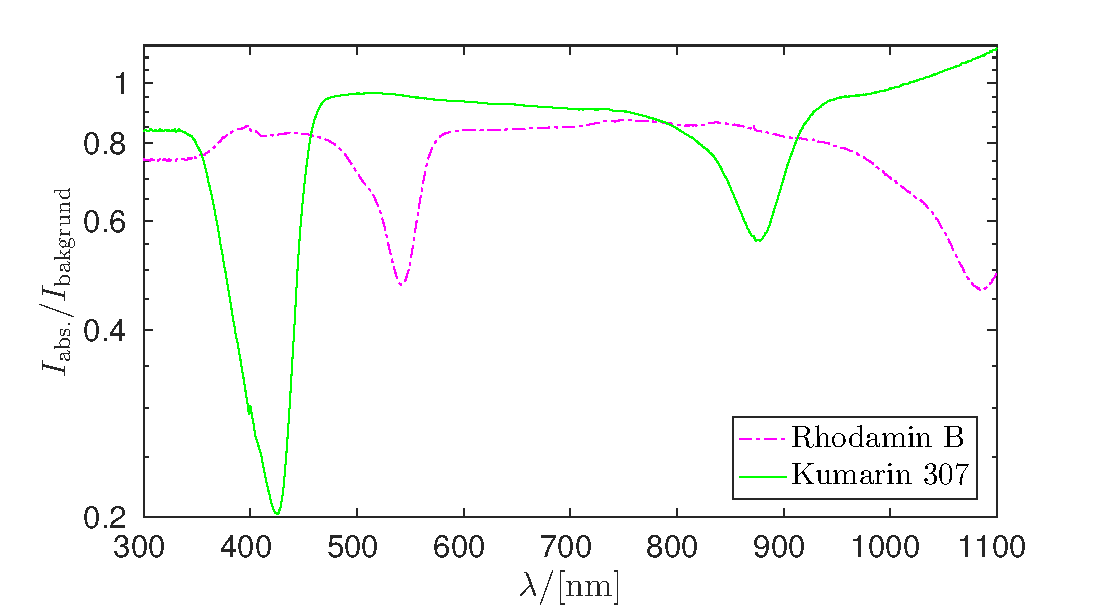
\includegraphics[width=.9\textwidth]{absorption.pdf}
}
\caption{Absorptionsspektrum från Rhodamin B och Kumarin
  307. Absorptionsspektrumen är framtagna som kvoten mellan
  intensiteten som lyste igenom provet mot intensiteten från samma
  ljuskälla utan något prov. Spektrat från glödlampan som användes som
  ljuskälla visas i \figref{fig:svartkropp} i Bilaga~\ref{sec:korr}.
}
\label{fig:absorption} 
\end{figure}

\section{Diskussion}
Överlag verkar laborationen vara ganska lyckad. Mycket av resultaten
stämmer överens med tidigare kända värden.
% I uppgiften med att identifiera energinivåerna i en atom nämndes att
% det är lätt att identifiera de olika energinivåernas inbördes avstånd,
% men att det kan bli svårt att bestämma de absoluta energierna. 


% Andra förväntade resultat för mätningen av laserfärgämnena är som
% nämnts tidigare att de kommer att sakna distinkta toppar och att de
% flourescerar med längre våglängder än det absorberar. 
\subsection{Spektrometern}
Spektrometern var som sagts tidigare en halvautomatisk maskin som
kunde styras tämligen enkelt från ett LabVIEW-program. Man bör i
sådana sammanhang vara extra försiktig och inte förledas att tro på
allt maskinen ger ifrån sig. Man ska även själv försöka undersöka vad
för bergränsningar som finns. 

\subsubsection{Upplösning i spektrometern}
\label{sec:diskussion_upplosning}
Spektrometern, Spex~270M, har en enligt tillverkaren \cite{Spex270M}
en våglängdsupplösning på $\Delta\lambda=\unit[0,1]{nm}$. Men den
faktiska upplösningen beror i högsta grad på vilka inställningar man
använder; i synnerhet beror upplösningen på spaltbredden för det
insläppta ljuset. 

I mätningarna på kvicksilverspektrat, där våglängdsupplösning är av
stor betydelse, användes därför den minsta spaltbredd som tilläts av
spektrometern. Det är alltså rimligt att anta att våglängsupplösningen
i mätningarna var samma som tillverkaren angav.

För att relatera detta till upplösning i energinivåerna\footnotemark{}
kan vara mer intressant att studera den relativa upplösningen,
$\Delta\lambda/\lambda$. Den kommer att variera för olika våglängder,
men man får en övre begränsning genom att ta den minsta våglängd som
man använder. Detta ger, med lite extra säkerhetsmarginal, att 
\[ 
\frac{\Delta\lambda}{\lambda}\le 0,05\,\%. 
\]
Detta kan, och görs i avsnitt~\ref{sec:diskussion_energi}, jämföras
med avvikelserna i \tabref{tab:Hg_nivaer}.
\footnotetext{Eftersom $\delta E\propto \lambda^{-1}$ blir
  $\frac{\Delta(\delta E)}{\delta E} = \frac{\Delta\lambda}{\lambda}$.}


\subsubsection{Våglängdskalibreringen}
En annan möjlig orsak till fel i kvicksilverspektrat är
våglängdskalibreringen. Den gjordes bara mot en punkt
(i Na-dubbletten). Det kan hända att spektrometern är byggd så bra att
det bara behövs. Men i princip hade det varit bättre om man kunde
kalibrera spektrometern mot åtminstone två punkter, för att upptäcka
om våglängdsstegen som spektrometern tar, faktiskt motsvarar samma
steg i verklig våglängd. 

Man kan dock indirekt se den goda överensstämmelsen med NITS:s data, i
både \tabref{tab:Hg_nivaer} och den lägre delen av spektrat i
\figref{fig:Hg_spektrum}, som en indikation på att enpunktskalibreringen
var tillräcklig.  

\subsubsection{Intensitetsmätning} 
Hittills har bara aspekter av spektrometern som berör
kvicksilvermätningar påtalats, men för absorptionsspektrumet kan det
vara intressant att studera hur väl spektrometern mäter inensitet. Här
kommer vi nu gå igenom några aspekter rörande intensiteterna. I
Bilaga~\ref{sec:korr} finns ytterligare material på detta område. 

Jämför man det uppmätta och det teoretiska spektrat
från en glödlampa finner man att spektrometern har en högsta
känslighet ungefär i våglängdsområdet 400--800\,nm. Detta kan ses i
figurerna~\ref{fig:svartkropp} och \ref{fig:korrektionsfaktor} i
Bilaga~\ref{sec:korr}. För att kompensera för den varierande
känsligheten beräknades en korrektionsfaktor som varierade från 1 upp
till omkring 100.
Detta föranleder bland annat att mätningar
utanför detta område bör betraktas med försiktighet -- en topp där kan
ha varit brus som gick över tröskeln och blev förstorat av
korrektionsfaktorn. 

Den huvudsakliga orsaken till det branta tappet i uppmätt intensitet
för våglängder högre än ca 800\,nm beror med största sannolikhet på
fotomultiplikatorns känslighetsområden. Eftersom fotomultiplikatorer
bygger på den fotoelektriska effekten kommer det finnas en viss minsta
fotonenergi som krävs för att slå ut en elektron i det första
steget. Det är troligtvis det som orsakar nämnt tapp i
känslighet för långa våglängder. Att känsligheten går ner i den
kortvågiga ändan är däremot märkligare och kräver en annan
förklaring. 

I fallet med mätningarna på absorptionsspektrat är detta dock inga
problem. Detta eftersom den uppmätta absorptionen mättes genom att
undersöka \emph{kvoterna} mellan intensiterna. Detta gör att
korrektionsfaktorn försvinner, och fotomultiplikatorn känslighet inte
påverkar resultatet i \figref{fig:absorption}.

% Vidare bör även mätningar över denna kritiska våglängd
% betraktas med försiktighet. Detta för att den fotoelektriska effekten,
% teoretiskt, inte över huvud taget borde fungera för fotoner med för
% lång våglängd. 

\subsection{Kvicksilverspektrum}
Man kan notera att de topparna med kortast våglängd i spektrumet kom i
ett kluster om tre, tätt liggande toppar. Detta tyder enligt
resonemanget i avsnitt~\ref{sec:teori_nivaer} på att spektrumet inte
omfattde några övergångar till kvicksilvers grundnivå,
$6^1\mathrm{S}_0$. Därför är det motiverat att anta att att alla andra
detekterade övergångar har skett mellan nivåer ovanför (och till)
$6^3\mathrm{P}_0$ som är det lägsta exciterade tillståndet. Så är
också fallet i den här rapporten.

\subsubsection{Diskreptans i spektrumet}
Som man kan se i \figref{fig:Hg_spektrum} så fattas många av topparna
som NIST \cite{NIST_spectrum} anger borde finnas. Vidare stämmer inte
intensiteterna helt överens med alla toppar. 

\paragraph{Missade toppar}
En möjlig anledning till att det fattas toppar kan ha varit att
metoden som användes för att ta upp spektrumen gick med stora steg
tills en topp detekterades. Alltså att toppar missades på grund av att
de stora stegen. Men upptagningen av spektrumet gjordes flera
gångar; vilket borde ha lett till att om det missades någon topp i
någon av mätningarna, så borde den ha kunnat fångas upp av en annan
mätning. 

Vidare så sattes tröskelvärdet så lågt att allt som stack över
bakgrundsbruset fångades upp. Och eftersom de starkare topparna blödde
ut kring bottnen av toppen så att intensiteten var över tröskelvärdet
under ett intervall som motsvarade flera av de längre steglängderna,
borde alla toppar som fanns i lampan som användes ha detekterats. Det
är alltså inte troligt att mätmetoden orsakade några bortfall av
spektraltoppar. 

I \cite{NIST_spectrum} finns det utöver ''strong lines'' även en
kategori som kallas ''persistent lines''. Denna andra kategori
innehåller en lista över de spektrallinjer som fins kvar även om det
förekommer föroreningar i provet. Denna lista inehåller betydligt
färre antal toppar. De toppar som finns med i listan\footnotemark{}
finns också med i \figref{fig:Hg_spektrum}, så av de topparna verkar
inga ha missats i våra mätningar. Det är alltså tänkbart att alla
''strong lines'' inte fanns med för att det förekom föroreningar i
spektrallampan, men att föroreningarna var så små att alla de känsliga
topparna inte påverkades. 
\footnotetext{Som ligger i intervallet 400--800\,nm.}


\paragraph{Intensitetsavvikelser}
Studerar man \figref{fig:Hg_spektrum} ser man att det finns en god
våglängdsöverensstämmelse mellan identifierade och tabellerade toppar
i det neder delen av spektrat, men intensiterna passar
sämmre. Detta är lite anmärkningsvärt men inget att oroa sig allt för
mycket över.

Eftersom jämförelsen här är mellan absoluta intensiteter kommer
fotomultiplikatorn känslighet att påverka mätningarna. Nu visas
förvisso de korrigerade intensiteterna i \figref{fig:Hg_spektrum}, men
det är tämligen osäker om korrektionsfaktorn stämmer. För vidare
diskussion om detta, se Bilaga~\ref{sec:korr}. 

För energinivåernas del är det bara varje topps våglängd som
påverkar. Så vad för intensitet topparna har är egentligen inte
inressant, vilket betyder att avvikelser i intensitet bara ska ses som
en fingervisning om hur väl mätningarna stämmer överens med
NIST:s \cite{NIST_spectrum} värden.

\subsubsection{Energinivåerna}\label{sec:diskussion_energi}
Det listade energinivåerna i \tabref{tab:Hg_nivaer} har en
anmärkningsvärt god överensstämmelse med NITS:s
\cite{NIST_levels}. Detta talar för att våglängsupplösningen som
beräknades i avsnitt~\ref{sec:diskussion_upplosning} verkar vara den
avgörande källan till osäkerhet. 

Det finns dock ett iögonfallande utstickande värde: det för
$7^1\mathrm{S}_0$ som skiljer sig från \cite{NIST_levels} med hela
2,74\,\%. Det är dessutom extra anmärkningsvärt eftersom den
energinivån beräknades från övergången 
$7^1\mathrm{S}_0 \to 6^3\mathrm{P}_0$ som ger en av de starkaste
topparna, vid ungefär 407\,nm. Det finns dessutom inte andra möjliga
kandidater kring den våglängden. Det borde inte ha blivit fel här helt
enkelt, men även de andra mätningarna ger att toppen ligger vid den
våglängden. 

De övriga energinivåernas goda överensstämmelse verkar dock peka på
att mätnigarna i övrigt var riktiga. Och att det relativa felet i
energier begränsas av våglängdsupplösningen\footnotemark{}
\[
\frac{\Delta E}{E} \sim \frac{\Delta\lambda}{\lambda} \le 0,05\,\%.
\]
\footnotetext{Egentligen kommer osäkerheterna i varje enskild
  energinivå att variera beroende på hur många övergångar man måste
  använda för att komma till den energinivån från
  $6^3\mathrm{P}_0$. Men detta ger en bra uppskattning om felets
  storleksordning. }

\subsubsection{Ej använda toppar 
               och eventuella oklarheter bland energinivåerna}

Som kan ses i \tabref{tab:Hg_toppar} i Bilaga~\ref{sec:kompl} så
användes bara ungefär hälften av de observerade topparna. Dessutom var
det främst de topparna med kortast våglängd som användes. Detta är
framför allt för att de långvågiga topparna svarar mot små steg
mellan energinivåer, och att ju högre upp i energinivå man kommer
destu tätare ligger nivåerna. Detta gör att det för de korta
våglängderna oftast finns många möjliga kandiadater. Detta gör det
svårt att vara säker på vilka nivåer en viss topp gäller. 

Det finns faktiskt redan en sådan konflikt bland de längre
våglängderna. Det är mellan $6^3\mathrm{D}_1$ oc $6^1\mathrm{D}_2$,
som enligt \cite{NIST_levels} bara skiljer sig med 1\,meV som är
mindre än osäkerheten som uppstår från våglängdsupplösningen. Vad
detta betyder är egentligen att dessa mätningar inte kan urskilja
dessa två nivåer, varför de båda kan betraktas ha samma energi i den
här rapporten. 


\subsection{Laserfärgämnenas absorptionsspektrum}
%Varför breda dalar och inte skarpa spikar?
%Varför har kumarin högre absorptionsförmåga?
%varför går intensiteten upp efter absorptionsdalen?

Figur \ref{fig:absorption} visar uppmätt absorptionsspektra för
laserfärgämnena rhodamin~B och kumarin~307. Vi påminner om viss
försiktighet vid betrakande av ändarna på spektrat eftersom
fotomultiplikatorn verkar vara som okänsligast i detta område. Därför är
resultatet från den vänstra delen av spektrat mest pålitligt. 


En intressant iaktagelse är att den andra absorptionsdalen, för båda
ämnena, ligger vid ungefär dubbla våglängden jämfört med den
första. Detta kan eventuellt bero på någon form av resonans i
molekylen -- jämför övertoner i en sträng. Resonansen skulle alltså du
kunna ge upphov till mellanliggande nivåer som orsakar absorption vid
halva energin. 

I samtliga fall har vi att göra med breda spektrala
absorptionsband. Förklaringen består delvis av att dessa
laserfärgämnen utgörs av stora organiska molekyler vilka som följd har
ett stort antal interna frihetsgrader i form av vibrations- och
rotationstillstånd. Dessa breda absorptionsband och motsvarande
emissionsband, som allmänt är förskjutna åt höger genom så kallat
Stokes-skift, kännetecknar ämnen som är flourescenta. 

Stokes-skiftet tycks förklara de högre trösklarna som syns efter varje
absorptionsdal, där ljuset emitteras längs alla rumsliga riktningar
och i våglängder som är en aning rödskiftade från
absorptionsvåglängderna. Tröskeln för Kumarin 307 är högre än den för
Rhodamin B och orsakas sannolikt av att Kumarin absorberar en större
mängd energi än Rhodamin B. 

Om vi haft mer tid att studera dessa laserfärgämnen hade det varit
intressant att undersöka ämnenas emissionsspektra samt hur känsliga
ämnena är för fotoblekning.



% För undersökningen av absorption i lösning har vi på förhand inte så
% mycket att utgå från. Vi har åtminstone att lösningsmedlet lär påverka
% energinivåerna i molekylen/jonen. Tidigare resultat för olika
% organiska färgämnen påvisar ett frekvensskift av absorptionstoppen
% beroende på hur polärt lösninsmedlet är \cite{Mannekutla2008}, men
% olika lösningmedel kan även starkt påverka absorptionens intensitet
% \cite{Homocianu2011}.
% I övrigt finns det annat som kan påverka absorptionsspektrat som
% exempelvis jonladdning om man undersöker metalljoner i lösning. 




\section{Sammanfattning}
Sammanfattningsvis kan vi konstatera att det gick bra
att ta upp olika typer av spektrum med den spektrometer som
användes. Detta ledde sen till att energinivåerna för
kvicksilveratomen kunde identifieras och bestämmas med förvånansvärt
hög överensstämmelse med tidigare data. 

Resultaten visar också hur
spektrumen skiljer sig dramatiskt mellan olika typer av prov. Atomära
spektrum uppvisar distinkta spektrallinjer. Medan spektrum från större
molekyler har betydligt bredare excitationsområden, vilket beror på
det stora antalet tättliggande energinivåer i vad som kan betraktas
som ''energiband''. 




%För att lägga in en referens så ska den skrivas in enligt mönstret i filen referenser.bib
%Använd \cite{} som vanligt för att använda referensen i texten.
%Här är en bra länk om hur man ska göra:
%https://en.wikibooks.org/wiki/LaTeX/Bibliography_Management#biblatex
\newpage
\iflanguage{swedish}{\renewcommand{\refname}{Källförteckning}}{}
\bibliographystyle{ieeetr}
\bibliography{referenser}


%Detta ser till att bilagorna kommer in snyggt i rapporten/förstudien
\clearpage
\appendix
%\setcounter{section}{0}
%\renewcommand{\thesection}{\Alph{section}}
\setcounter{page}{1}
\renewcommand*{\thepage}{A\arabic{page}}
\phantomsection{}
\iflanguage{swedish}{\renewcommand{\appendixname}{Bilagor}}{}
\addcontentsline{toc}{part}{\appendixname}
\iflanguage{swedish}{\renewcommand{\appendixname}{Bilaga}}{}




\section{Teoribakgrund} \label{sec:teori}
I den här bilagan presenteras delar av den teori som behövs för att
bestämma energinivåer på egen hand. I den här rapporten används dock
en referenstabell för att passa in de toppar från det uppmätta
spektrumet till redan tidigare bestämda energinivåer. Detta gör mycket
av den här bilagan överflödig för rapportens skull, men om man inte
hade haft några tidigare referenser måste man använda vad som
presenteras här (och lite till).

\subsection{Spektroskopins grundläggande idé}
Elektroner är bundna till atomkärnan i väldefinierade kvanttillstånd
kallade atomorbitaler. Varje sådant tillstånd har en väldefinierad
energi. Elektroner kan röra sig mellan energinivåerna genom att
absorbera eller emittera en foton med energi som matchar 
energiskillnaden mellan atomens orbitaler. 

En elektron kan ''hoppa'' till ett högre energitillstånd genom att
absorbera en foton som motsvarar den energi som krävs för nå en högre
energinivå. Man säger då att elektronen exciteras genom att
\emph{absorbera} en foton. Vid övergång från ett högre till lägre
energitillstånd \emph{emitteras} istället en foton med den frekvens
som svarar mot energiskillnaden mellan energinivåerna. 
 
% Varje grundämne karakteriseras av en unik sammansättning av
% elektroner och orbitaler som är bundna till kärnan i unika
% konfigurationer. Detta leder till att energinivåerna är unika för
% varje grundämne varför spektroskopi är ett kraftfullt verktyg för
% ämnesbestämming. 
 
Genom att studera vilka ljusvåglängder som emitteras från ett prov
kan alltså de olika energiskillnaderna bestämmas med hjälp av  
\[\delta E = h\nu=\frac{hc}{\lambda}.\]
På så sätt kan alla energinivåer (med $\delta E$ i de detekterbara
våglängderna) bestämmas relativt varandra. 

Att bestämma de absoluta
energierna på varje nivå är däremot svårare. Det bästa man kan hoppas
på är att bestämma de exciterade energinivåerna relativt
grundtillståndet eller kanske rent av relativt första exciterade
nivån. Det är nämligen troligt att grundtillståndet ligger betydligt
lägre än de oftast mer tätliggande exciterade nivåerna. 

\subsection{Kvanttal och elektronskal}
Kvantmekaniskt beskrivs de olika orbitalerna av i huvudsak två
kvanttal. Det ena kallas huvudkvanttalet, $n$, och styr vilka andra
kvanttal som är tillåtna. Det andra är det azimutala kvanttalet, $l$,
som beskriver banrörelsemängdsmomentet en elektron med det kvanttalet
har. 

Vidare finns även det magnetiska kvanttalet, $m$, och spinnkvanttalet,
$s$. Som namnen antyder så kommer $m$ in i situationer med magnetfält,
exempelvis Zeemaneffekten, och $s=\pm\nicefrac{1}{2}$ bestämmer
elektronens spinn. 
Av dess är det bara spinnkvanttalet som kommer vara av intresse för
den här rapporten.  

Med Paulis uteslutningsprincip kan man sedan bygga upp elektronskal
som fylls upp med elektroner för större grundämnen. Skalen i dessa
atomer fylls på nerifrån, i energi räknat. Detta leder till att det
kommer finnas elektroner i fyllda och ofyllda skal. För (optisk)
spektroskopi är de elektroner i fyllda skal ointressanta, då de är
mycket hårdare bundna till kärnan än valenselektronerna, de yttersta
elektronerna, som lättare kan exciteras. 



\subsection{Spektroskopiska termer}\label{sec:term}
Man brukar alltså bara intressera sig för valenselektronerna och deras
tillstånd. Men när man har flera elektroner i en atom räcker det
tyvärr inte att bara titta på valenselektronernas konfiguration. För att
få det sammanlagda tillståndet, som även bero på hur de olika
elektronerna Coulomb-växelvärkar med varandra, använder man sig av så
kallade \emph{LS-termer} eller \emph{spektroskopiska termer}.

Dessa spektroskopiska termer är uppbyggda enligt formen \cite{Bransden}
\[
^{2S+1}L_J,
\]
där $S$ är de möjliga kombinatinoer av de båda elektronernas
spinnkvanttal, $L$ antar heltalsvärden från skillnaden till summan av
de båda elektroneras azimutala kvanttal, det samma för $J$ fast med
$L$ och $S$ istället. Detta kan för två valenselektroner sammanfattas
med formlerna \cite{Bransden}
\begin{equation*}
\begin{aligned}
L &= |l_1-l_2|, |l_1- l_2|+1, \ldots, |l_1+l_2|\\
S &= |s_1-s_2|, |s_1- s_2|+1, \ldots, |s_1+s_2|\\
J &= |L-S|, |L-S| +1, \ldots, |L+S|,
\end{aligned}
\end{equation*}
där indexen betecknar att kvanttalen hör till respektive elektron.

När termerna skrivs ut används den spektroskopiska beteckningen (S, P,
D, o.s.v.) för $L$. Vidare använder man $2S+1$ i termen vilket är för
att det ger antalet olika termer med samma $L$ och $S$ -- om inte
$L=0$. Detta gör att termer med $S=0$ och med $S=1$ kallas singeltt-
respektive triplettillstånd. 

\subsection{Spinn-bankoppling}\label{sec:LS}
Om man ska använda dess termer som svarar mot en uppsplittring av energinivåerna
jämfört med enelektronsystem, så bör man ha koll på vilken typ av uppsplittring
som sker. Det finns i huvud sak två olika sorteras uppsplittringar som motsvarar
olika typer av kopplingar mellan elektronerna, LS- eller jj-koppling. 

Båda hänger på den å kallade spinn-bankopplingen. Det viktigaste med
spinn-bankopplingen är hur stor uppsplittringen blir. Detta för att kunna
uppskatta ungefär hur tätt olika energinivåer ligger. Spinn-banuppsplittringen
går som\cite{Bransden} 
\[
\Delta E_\text{SB} \propto Z^4 \ev{\frac{1}{r^3}},
\]
där $Z$ är atomnumret och $r$ är elektronens avstånd från kärnan.

I fallet med höga atomnummer och starkt positivt joniserade atomer, så är
spinn-banväxelverkan mest framträdande. Då beräknas först
spinn-banuppsplittringen och sedan läggs Coulomb-växelverkan in som en
finare uppsplittring av energinivåerna. Detta kallas för
jj-koppling. Man kan lätt se att det blir så för stora $Z$ eftersom
spin-banväxelverkan går som $Z^4$, men för neutrala atomer blir den
effektiva kärnladdningen mindre eftersom de inre elektronerna skärmar
av kärnladdningen för valenselektronerna. 

Om Coulomb-växelverkan mellan valenselektronerna däremot är stor
jämfört med spinn-banväxelverkan (spinn -- S, banrörelsemängdsmoment
-- L), så kan man börja med att räkna fram uppsplittringen från
Coulomb-växelverkan och sedan lägga på sipnn-ban-växelverkan. Detta
ger en uppsplittring i först $^{2S+1}L$ och sedan en mindre
uppsplittring i $J$. Detta kallas för LS-koppling. 

I den här rapporten antas LS-koppling råda för
kvicksilveratomerna. Detta är som nämnts tidigare en ganska bra
approximation för neutrala atomer, men även det faktum att $\Delta
E_\text{SB} \propto \ev{r^{-3}}$ bidrar till att göra
spinn-banväxelverkan liten. 



\subsection{Regler för underlättande av energinivåövergångsindentifiering} 
\label{sec:regler}
För att underlätta identifieringen av övergångar kan man försöka
sortera upp energinivåerna efter vilken energi de har. Här kan man
börja med att använda den så kallade \emph{Aufbau principen} eller
\emph{Madelungregeln} som tumregel för i vilken ordning orbitalerna
ska fyllas\cite{wiki:aufbau}. Principen säger att de orbitaler med 
lägst $n+l$ har lägst energi, med fördel för lägsta $n$ om $n+l$ är
lika. Detta är bara en tumregel och ska inte tas stenhårt, men det 
är ändå ett bra hjälpmedel. Dessutom gäller den bara för neutral 
atomer i sitt grundtillstånd så egentligen gäller den inte i de här
situationerna, men det är bara som sagt en tumregel.

För att avgöra den inbördes ordningen mellan termer hörande till samma
konfiguration finns de så kallade \emph{Hunds regler} \cite{Bransden}. 
\begin{enumerate}
    \item Större $S$ ger lägre energi.
    \item För ett givet värde på $S$ så har den term med störst $L$ lägst energi
    \item 
    \begin{enumerate}
        \item Mindre än halvfullt skal ger minst energi för \emph{minsta} $J$.
        \item Mer än halvfullt skal ger minst energi för \emph{störst} $J$.
    \end{enumerate}
\end{enumerate}

Ett hjälpmedel i bestämmandet av energinivåerna är de så
kallade \emph{urvalsreglerna} som bygger på hur en elektrisk dipol kan
växelverka med elektronerna. De bestämmer vilka övergångar mellan
tillstånd som är tillåtna vid vid växelverkan (absorption eller
emission) med fotoner. För LS-koppling är de regler som är mest intressanta:  
\begin{equation*}
\begin{aligned}
\Delta L &= \pm 1 \\
\Delta J &= 0, \pm 1 \quad (J=0\to 0\text{, är inte tillåtet})
\end{aligned}
\end{equation*}
som styr hur $L$ och $J$ kan förändras vid dipolväxelverkan
\cite{Bransden}. Egentligen kan även $\Delta L=0$, men den här
rapporten kommer enbart  behandla tillstånd där en elektron har
exciterats från grundtilståndet. Detta gör att eftersom den elektronen
som exciterats måste ha ett $\Delta l_i =\pm 1$ \cite{Bransden} så
måste även $L$ ändras lika mycket. 







\section{Intensitetskorrektion}\label{sec:korr}
Som kan ses i \figref{fig:svartkropp} finns en diskrepans mellan
formen på det uppmätta sprektrat och vad Plancks strålningslag
förutspår. Detta leder till att topparnas höjd i
\figref{fig:Hg_spektrum} inte motsvarar deras faktiska
intensitet.\footnotemark{} Detta gör det svårt att jämföra dessa
mätningarna mot andras resultat. För att ändå kunna göra sådana
jämförelser beräknades korrektionsfaktor, $K$, så att
\[
I_\text{verklig}(\lambda) = I_\text{uppmätt}(\lambda) \cdot K(\lambda).
\]
\footnotetext{Den här effekten har däremot ingen påverkan på
  resultatet för absorptionsspektrat, eftersom det som visas i
  \figref{fig:absorption} är kvoten mellan intensiteterna med och utan
  proverna. }


\begin{figure}\centering
\centerline{ %centrerar även större bilder
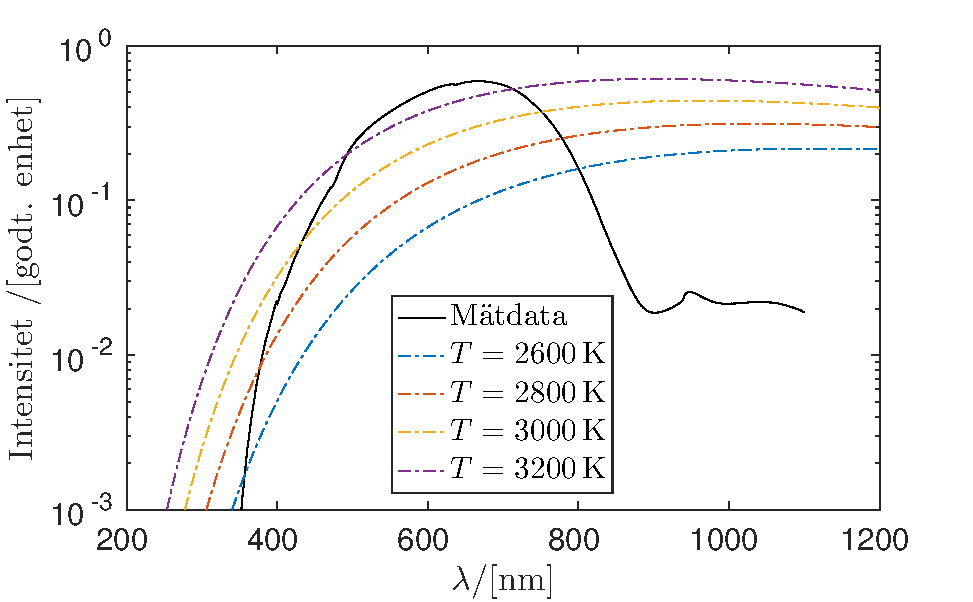
\includegraphics[width=.9\textwidth]{svartkropp.pdf}
}
\caption{Uppmätt spektrum (heldraget) med spektrometern från en
  glödlampa, jämfört med vad Plancks strålningslag ger (normerade
  kurvor). Härifrån syns tydligt att spektrometern har ett ganska
  snävt känslighetsområde där man helst inte bör gå mycket högre än
  till ca 800\,nm våglängd.}
\label{fig:svartkropp}
\end{figure}


\subsection{Temperaturkänslighet 
               och riktigheten i Plancksstrålingslag} 
Det räcker inte med att bara säga att man ska korrigera mätningarna
så att de passar till Plancks strålingslag. Man måste dessutom ange
till vilken temperatur av svartkroppsstrålning man ska anpassa. I det
här fallet valdes att anpassa till 3200\,K. 

I allmänhet hade en högre temperatur haft bättre passform till den
uppmätta spektralkurvan. Men eftersom det var en glödlampa så ligger
glödtrådens temperatur definitivt under 3700\,K, som är wolframs
smältpunkt. 

Så 3200\,K valdes lite godtyckligt, men det var den högsta troliga
temperaturern för glödtråden. Dessutom är den exakta temperaturen att
anpassa sin svartkroppsstrålning till inte så viktig. Detta syns i
\figref{fig:svartkropp} där \emph{formen} på kurvorna till de olika
temperaturerna varierar mycket lite mellan 2600--3200\,K. 

Vidare är det inte säkert att det går att använda Plancks strålingslag
rakt av. Den förutsätter en perfekt svartkropp, men det är inte säkert
att glödtråden har samma emittans i hela det anpassade spektrat. Det
bör dock inte vara ett jättestort problem eftersom de absoluta
inensiteterna inte är helt avgörande för resultaten i den här
rapporten. 


\subsection{Polynomanpassning och resultat}
Korrektionen som beräknas fram behöver kunna beräknas för en
godtycklig våglängd i mätintervallet eftersom de exakta våglängderna
som användes skiljer sig mellan mätningarna. Därför valdes att göra en
polynomanpassning som visas i \figref{fig:korrektionsfaktor}. 

I \figref{fig:korrektionsfaktor} visas de rena kvoterna och
anpassningen i logaritmisk skala, vilket är lite missvisande ur ett
numeriskt perspektiv. Det är nämligen mycket svårt att få med alla
detaljer i de områden där kvoten är liten när variationerna i värde
går över flera storleksordnigar. För att hantera detta problem gjordes
polynomanpassningen till den logaritmerade kvoten: 
\[
P_\text{anpassad} (\lambda) 
\approx \log(\frac{I_\text{Planck}}{I_\text{spektrometer}}).
\]
Detta leder alltså till att den faktiska korrektionsfaktorn blir
\[
K(\lambda) = \exp(P_\text{anpassad}(\lambda)),
\]
vilket är vad som visas i \figref{fig:korrektionsfaktor}.

Att göra en polynomanpassning är alltid en avvägning mellan å ena
sidan att få med så mycket detajer av kurvan som möjligt, och å andra
sidan inte få ett överanpassat polynom. Eller med andra ord hur hög
grad på polynomet man ska anpassa med. Överanpassade polynom får
bättre passning till de punkter som används, men kan resultera i en
sort oönskad svängning i ändpunkterna. 

Polynomet som användes i anpassningen i den här rapporten var av
grad~17. Gradtalet på anpassningspolynomet valdes genom att pröva sig
fram tills det såg ut att passa. Man kan dock redan här se antydningar
om överanpassning till höger i \figref{fig:korrektionsfaktor}, men de
ansågs vara så små och i ett intervall av mindre vikt så inget gjordes
åt dem. 

Det slutglitiga resultatet av korrektionen visas i
\figref{fig:anpassad_svartkropp}. Man kan se att den korrigerade datan
föjer Plancks strålningslag mycket väl utom i några enstaka
punkter. Det är dock inte så farligt, eftersom huvudsyftet med
korrektionen var att grovt kunna jämföra intensiteten på de
detekterade topparna med tidigare resultat. 

\begin{figure}\centering
\centerline{ %centrerar även större bilder
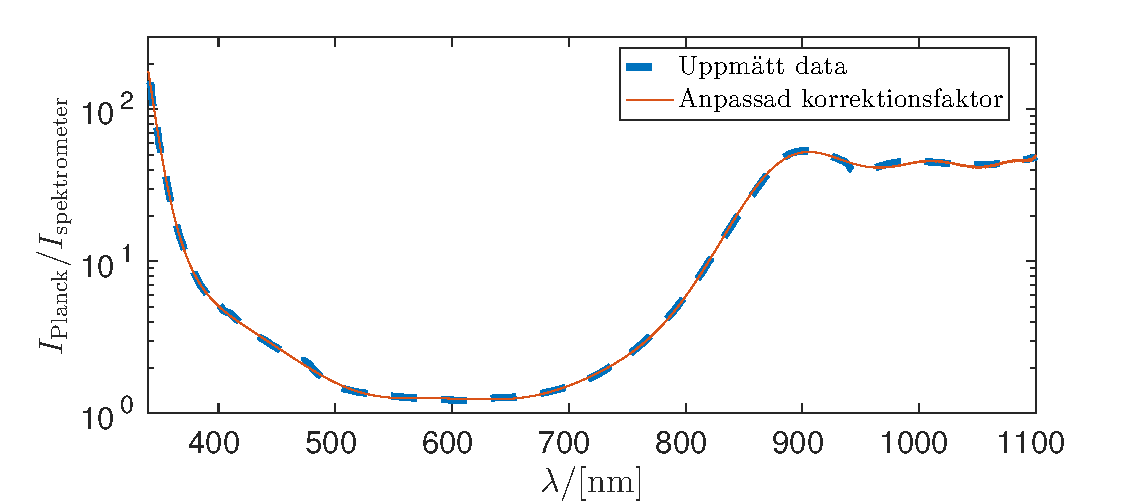
\includegraphics[width=.8\textwidth]{korrektionsfaktor.pdf}
}
\caption{Korrektionsfaktor från kvoten mellan uppmätta spektrumet från
en glödlampa och från Plancks strålningslag. Här visas även
polynomanpassningen som används i \figref{fig:Hg_spektrum}.}
\label{fig:korrektionsfaktor}
\end{figure}

\begin{figure}\centering
\centerline{ %centrerar även större bilder
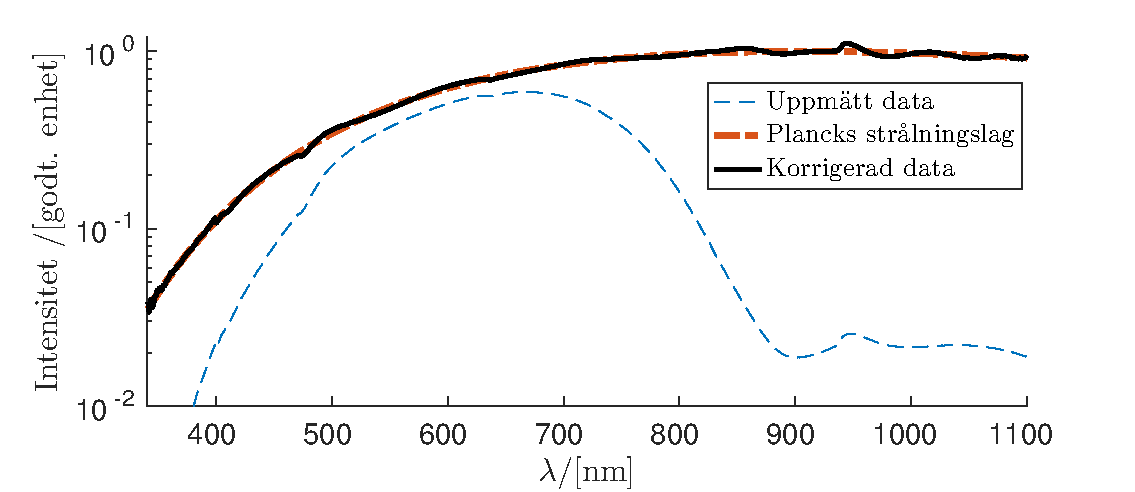
\includegraphics[width=.8\textwidth]{anpassad_svartkropp.pdf}
}
\caption{Jämförelse mellan uppmätt spektrum från en glödlampa och
  Plancks strålnigslag för en svartkropp på 3200\,K tillsammans med
  det korrigerade sprektrat. }
\label{fig:anpassad_svartkropp}
\end{figure}


\section{Kompletterande tabeller}\label{sec:kompl}
Här finns kompletterade, mer noggran presentation av data. Dessa tabellerna är inte väsentliga för rapporten, men kan vara till visst stöd ifall man är intresserad av att återupprepa något steg som presenterats.

I \tabref{tab:Hg_toppar} visas våglängder och motsvarande energier för topparna i \figref{fig:Hg_spektrum}. Dessa data används sedan för att rekonstruera energinivåerna i Hg.

\begin{table}
\centering
\caption{Tabell med uppskattad energiordning av LS-termer. Energin ökar uppåt i tabellen och inom samma rad så ökar även energin åt vänster. (Notera att singlettillstånden har skattats till högre energi än triplettillstånden.)} 
\label{tab:sorterade_termer}
\begin{tabular}{|c|ccc|}\hline
Singeltt & & Trippletter &\\\hline\hline
 $9^1\mathrm{S}_0$ & & &\\
&$9^3\mathrm{S}_1$ & --- &--- 
\\ \hline
 $8^1\mathrm{P}_1$ & & &\\
&$8^3\mathrm{P}_0$ & $8^3\mathrm{P}_1$ & $8^3\mathrm{P}_2$ 
\\ \hline
 $7^1\mathrm{D}_2$ & & &\\
&$7^3\mathrm{D}_1$ & $7^3\mathrm{D}_2$ & $7^3\mathrm{D}_3$ 
\\ \hline
 $6^1\mathrm{F}_3$ & & &\\
&$6^3\mathrm{F}_2$ & $6^3\mathrm{F}_3$ & $6^3\mathrm{F}_4$ 
\\ \hline
 $8^1\mathrm{S}_0$ & & &\\
&$8^3\mathrm{S}_1$ & --- &--- 
\\ \hline
 $7^1\mathrm{P}_1$ & & &\\
&$7^3\mathrm{P}_0$ & $7^3\mathrm{P}_1$ & $7^3\mathrm{P}_2$ 
\\ \hline
 $6^1\mathrm{D}_2$ & & &\\
&$6^3\mathrm{D}_1$ & $6^3\mathrm{D}_2$ & $6^3\mathrm{D}_3$ 
\\ \hline
 $7^1\mathrm{S}_0$ & & & \\
&$7^3\mathrm{S}_1$ &--- &--- 
\\ \hline
 $6^1\mathrm{P}_1$ & & &\\
&$6^3\mathrm{P}_0$ & $6^3\mathrm{P}_1$ & $6^3\mathrm{P}_2$ 
\\ \hline
$6^1\mathrm{S}_0$ & --- & --- & ---
\\ \hline
\end{tabular}
\end{table}



\begin{table}
\centering
\caption{Våglängder och energier för detekterade toppar (markerade med
  blå trianglar i \figref{fig:Hg_spektrum}) i Hg-spektrumet. } 
\label{tab:Hg_toppar}
\begin{tabular}{|c|c|c||l|}\hline
$\lambda$/[nm] & $\delta E$/[eV]  &$\delta E/[\unit[10^3]{cm^{-1}}$]
& Övergång\\ \hline
364,94  	& 3,397 	& 27,40
& $6^3\mathrm{D}_3\to 6^3\mathrm{P}_2$ 
\\ 
365,38  	& 3,393 	& 27,37 
& $6^3\mathrm{D}_2\to 6^3\mathrm{P}_2$ 
\\ 
366,19  	& 3,386 	& 27,31 
& $6^3\mathrm{D}_1\to 6^3\mathrm{P}_2$ 
  ($6^1\mathrm{D}_2\to 6^3\mathrm{P}_2$)
\\ 
390,50  	& 3,175 	& 25,61 
& $8^1\mathrm{D}_2\to 6^1\mathrm{P}_1$ %(?)
\\ 
404,69  	& 3,064 	& 24,71 
& $7^3\mathrm{S}_1\to 6^3\mathrm{P}_0$ 
\\ 
407,62  	& 3,042 	& 24,53 
& $7^1\mathrm{S}_0\to 6^3\mathrm{P}_0$ 
\\ 
433,75  	& 2,858 	& 23,05 
& $7^3\mathrm{D}_2\to 6^1\mathrm{P}_1$ %(?)
\\ 
434,50  	& 2,853 	& 23,01 
& $7^1\mathrm{D}_2\to 6^1\mathrm{P}_1$ %(?)
\\ 
435,62  	& 2,846 	& 22,96 
& $7^3\mathrm{S}_1\to 6^3\mathrm{P}_2$ 
\\ 
444,44  	& 2,790 	& 22,50 
& --- 
\\ 
546,00  	& 2,271 	& 18,32 
& $7^3\mathrm{S}_1\to 6^3\mathrm{P}_2$ 
\\ 
554,44  	& 2,236 	& 18,04 
& ---
\\ 
576,94  	& 2,149 	& 17,33 
& $6^3\mathrm{D}_2\to 6^1\mathrm{P}_1$ 
\\ 
578,94  	& 2,142 	& 17,27 
& $6^3\mathrm{D}_1\to 6^1\mathrm{P}_1$ 
  ($6^1\mathrm{D}_2\to 6^1\mathrm{P}_1$) 
\\ 
690,94  	& 1,794 	& 14,47 
& $8^3\mathrm{P}_2\to 7^3\mathrm{S}_1$ 
\\ 
730,31  	& 1,698 	& 13,69 & --- \\ 
731,25  	& 1,696 	& 13,68 & --- \\ 
732,81  	& 1,692 	& 13,65 & --- \\ 
781,44  	& 1,587 	& 12,80 & --- \\ 
809,44  	& 1,532 	& 12,35 & --- \\ 
815,94  	& 1,520 	& 12,26 & --- \\ 
872,00  	& 1,422 	& 11,47 & --- \\ 
983,88  	& 1,260 	& 10,16 & --- \\ 
\hline
\end{tabular}
\end{table}



\newpage
\stepcounter{section}
\phantomsection{}
\addcontentsline{toc}{section}{\Alph{section}\hspace{8 pt}Labblogg}
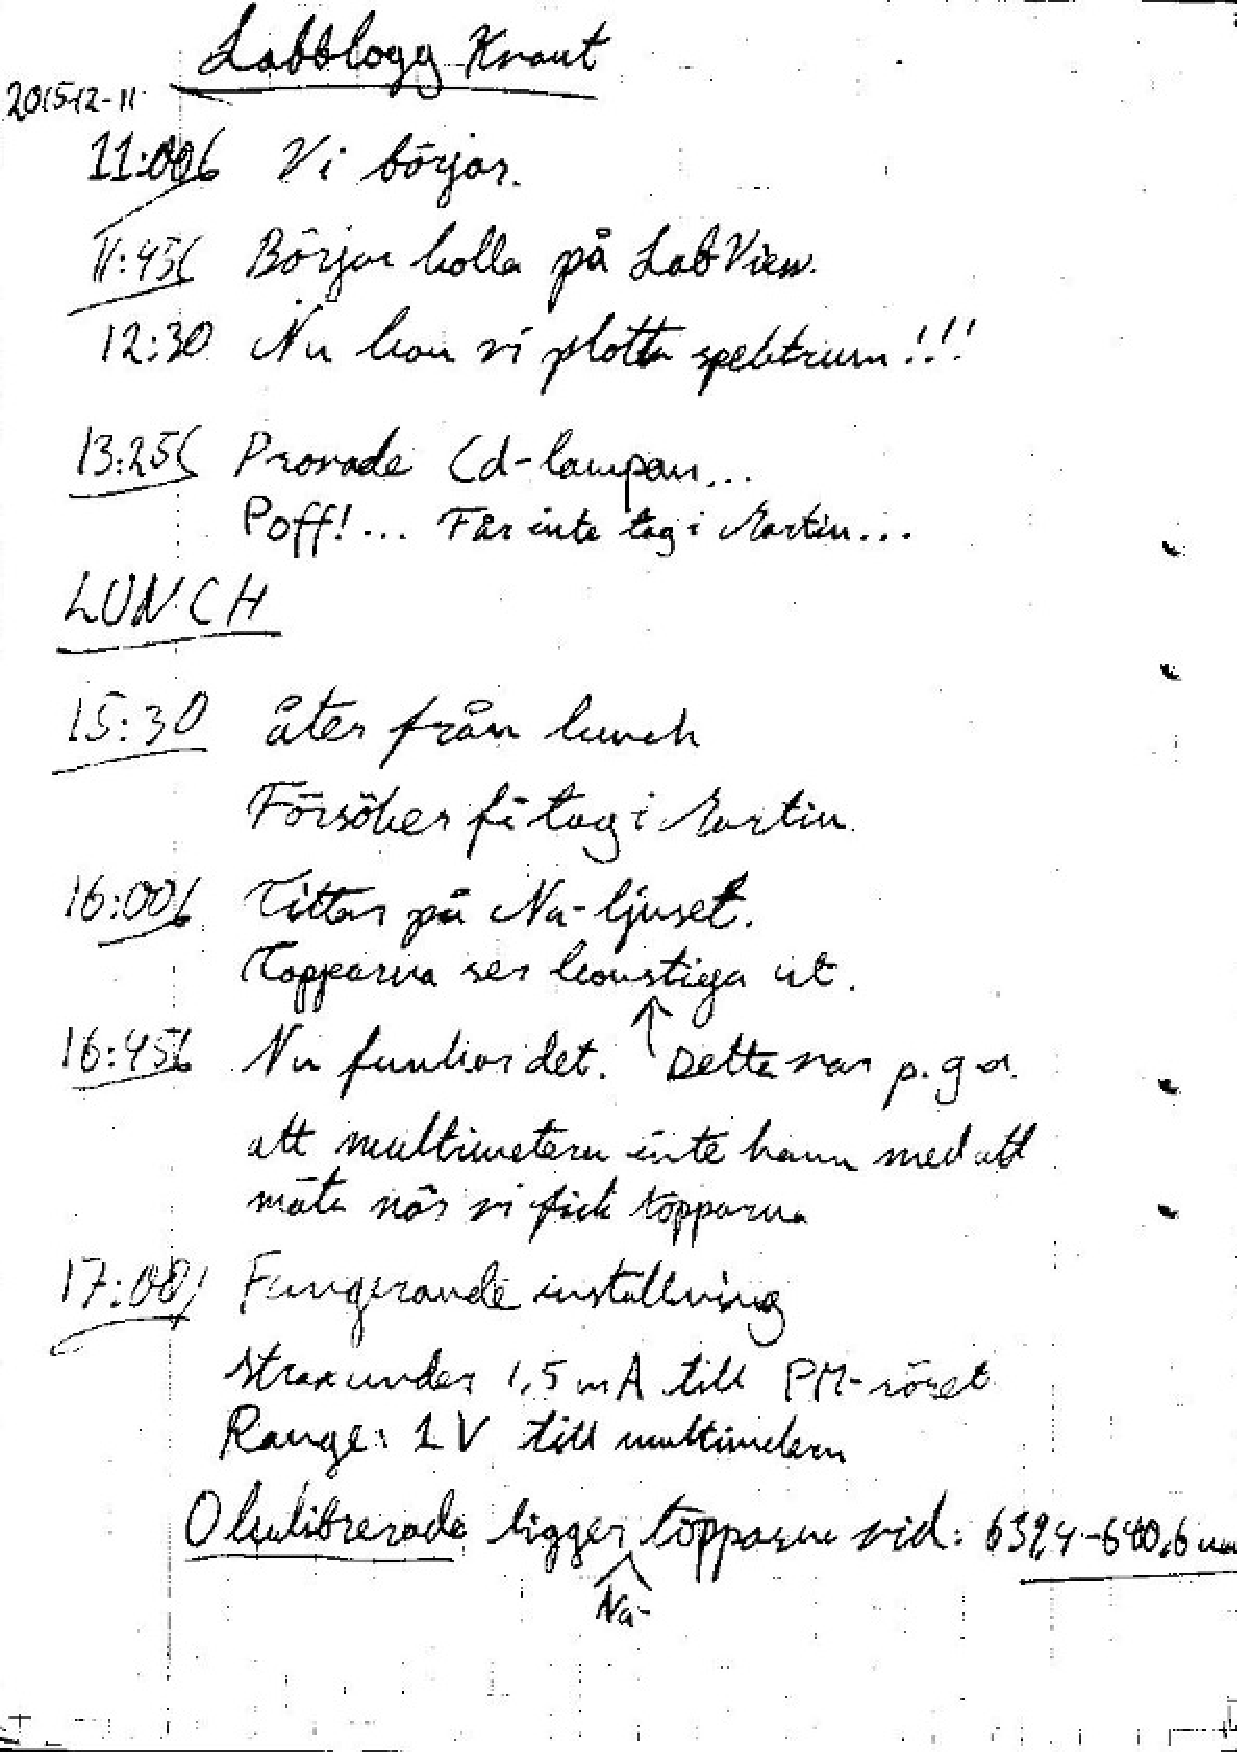
\includepdf[pages={1-}]{bilder/labblogg_kvant.pdf}


\end{document}


%% På svenska ska citattecknet vara samma i både början och slut.
%% Använd två apostrofer (två enkelfjongar): ''.

%%För att referera till till tidigare fotnot:
%    \footnotemark[\value{footnote}]

%% Figurer inkluderade som pdf-filer
%\begin{figure}\centering
%\centerline{ %centrerar även större bilder
%\includegraphics[width=1\textwidth]{filnamn.pdf}
%}
%\caption{}
%\label{figuren}
%\end{figure}

%% Figurer inkluderade med xfigs "Combined PDF/LaTeX"
%\begin{figure}\centering
%\input{filnamn.pdf_t}
%\caption{}
%\label{finafiguren}
%\end{figure}

% rhodamin b. Tusan. Vi gjorde extrauppgiften fel. https://www.akzonobel.com/colloidalsilica/system/images/AkzoNobel_Photo_cataytic_titania_coated_silica_spheres_tcm135-51192.pdf
